\newpage
\section{Part A}

\begin{figure}[htbp]
   \centering
   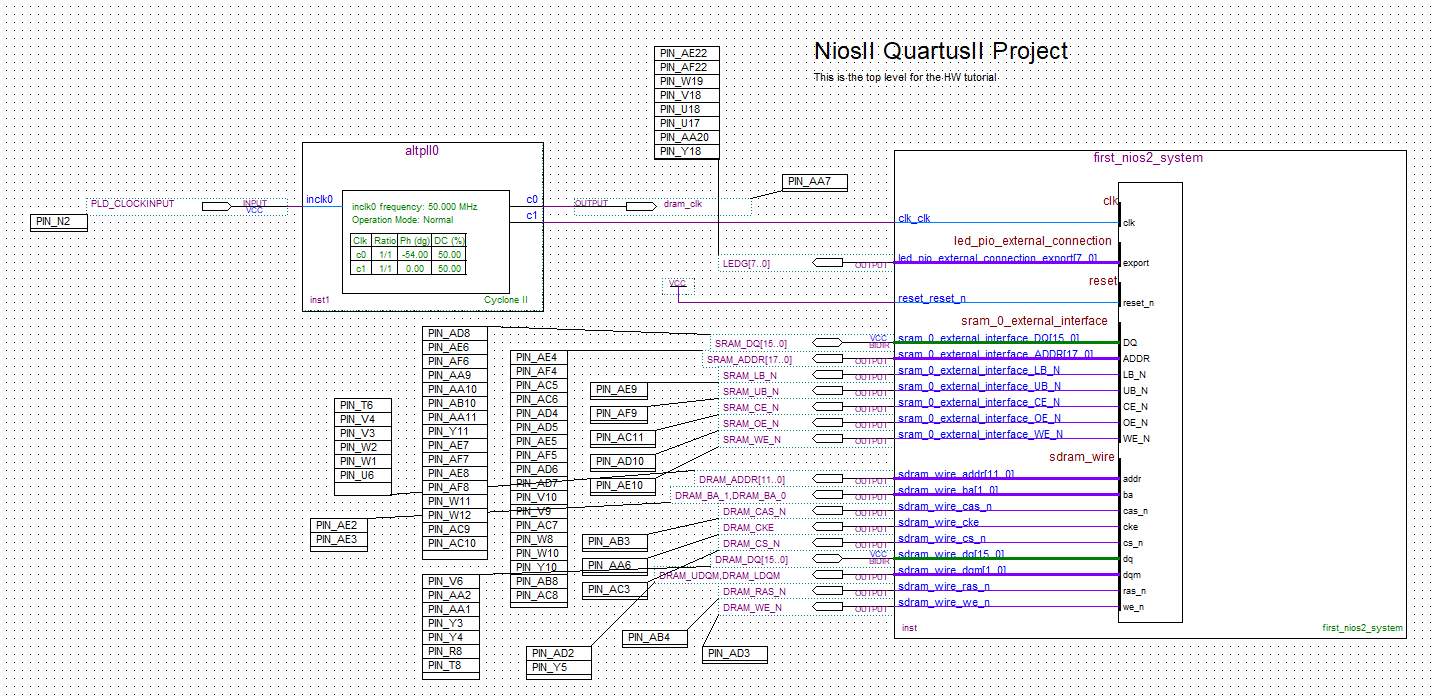
\includegraphics[width=0.9\textwidth]{block-diagram}
   \caption{Block diagram of the Nios II system}
   \label{fig:block-diagram}
\end{figure}

\begin{figure}[htbp]
   \centering
   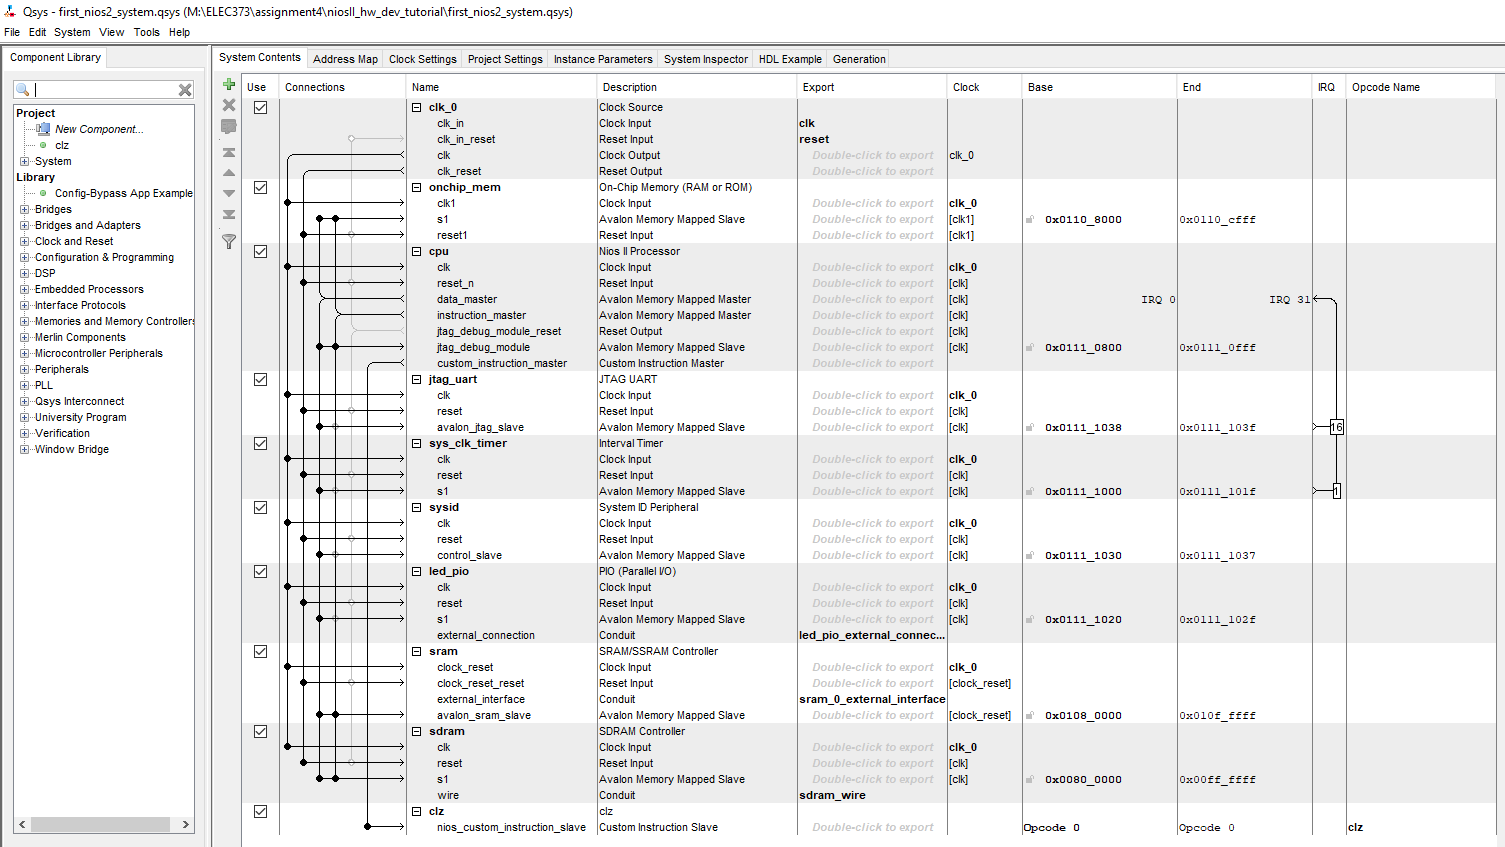
\includegraphics[width=0.9\textwidth]{memory-map}
   \caption{Nios II system contents}
   \label{fig:qsys}
\end{figure}

Figure \ref{fig:block-diagram} is the block diagram of the Nios II system. The system has a static RAM and dynamic RAM, as shown in Figure \ref{fig:qsys}. The static RAM was mounted to the FPGA's address from 0×0108000 to 0×010FFFFF. The dynamic RAM was mounted to the address from 0×00800000 to 0×00FFFFFF. The dynamic RAM's clock leads the CPU clock by 3 nanoseconds to meet the timing requirements by using the phase-locked loop (PLL).

To verify that both memories are working properly, the sample memory test code was run. The results are shown in Figure \ref{fig:part-a}.

\begin{figure}[htbp]
   \centering
   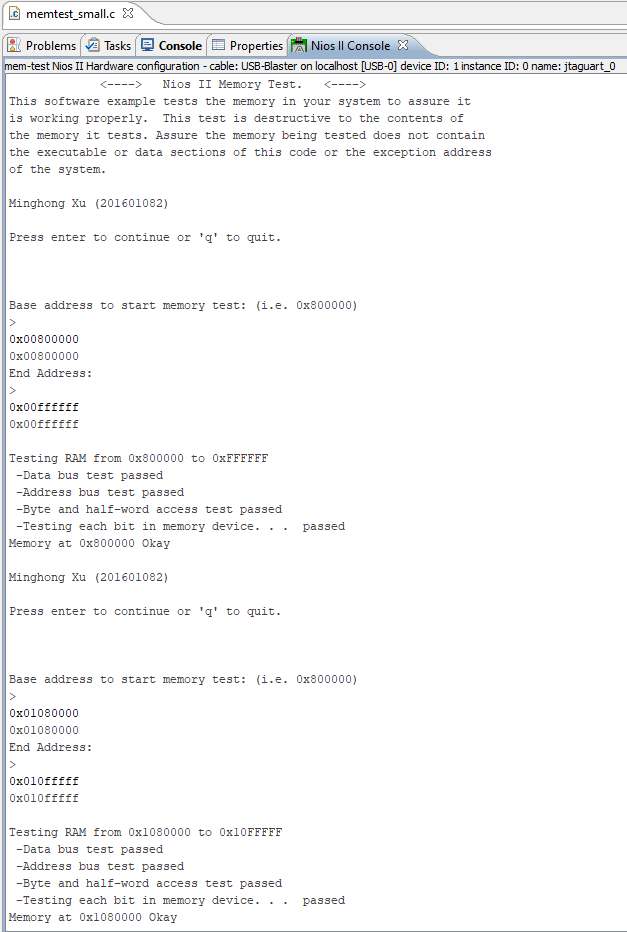
\includegraphics[width=\textwidth]{part-a}
   \caption{SRAM and SDRAM test passed}
   \label{fig:part-a}
\end{figure}
